\documentclass[conference]{IEEEtran}
\IEEEoverridecommandlockouts
\usepackage[T1]{fontenc}
\usepackage[utf8]{inputenc}
\usepackage{lmodern}
\usepackage{cite}
\usepackage{url}
\usepackage{booktabs}
\usepackage{array}
\usepackage{amsmath}
\usepackage{amssymb}
\usepackage{graphicx}
\usepackage{xcolor}
\usepackage{tikz}
\usetikzlibrary{positioning,arrows.meta,fit}
\usepackage{listings}
\lstset{basicstyle=\ttfamily\scriptsize,breaklines=true,columns=fullflexible,frame=single,aboveskip=4pt,belowskip=4pt}
\newcommand{\ac}{AC-DPP}
\begin{document}
\title{Towards Artisan-Centred Digital Product Passports:\\ Linking Material, Product, and Human Provenance Through Semantic Models}
\author{\IEEEauthorblockN{Author Name(s)}\IEEEauthorblockA{Institution / Research Centre\\City, Country\\email@institution.example}}
\maketitle
\begin{abstract}
Digital Product Passports (DPPs) are being developed to support product transparency, traceability, and circularity. For handcrafted products, however, knowledge of material origin and product transformations alone does not explain who made the product or how distinct makers contributed to its creation. This paper develops a research-grounded conceptual proposal for an Artisan-Centred Digital Product Passport (AC-DPP) that connects material, product, and artisan provenance through explicit activity and contribution records. An analytical review of DPP ontologies, general provenance standards, and digital craft heritage approaches informs an ontology-alignment strategy reusing PROV-O, CIDOC CRM, and concepts from the Crafts Ontology. We specify information requirements, a contribution-centred semantic pattern, illustrative competency questions, a layered system architecture, and an evaluation protocol. The approach distinguishes representation of a contribution from evidence supporting its authenticity and requires role-sensitive access to personal information. This is a conceptual design and evaluation agenda rather than a claim of an implemented or experimentally validated solution. The framework aims to facilitate item-level traceability while recognizing collaborative artisanal work and supporting craft-heritage documentation.
\end{abstract}
\begin{IEEEkeywords}
Digital Product Passport, artisan provenance, crafts, material traceability, PROV-O, CIDOC CRM, knowledge graph, semantic interoperability
\end{IEEEkeywords}

\section{Introduction}
Digital Product Passports (DPPs) are intended to make product-related information accessible and reusable across lifecycle stages and supply-chain participants. The European Union's Ecodesign for Sustainable Products Regulation (ESPR), Regulation (EU) 2024/1781, provides a framework for product-group-specific DPP requirements, including persistent product identifiers, data carriers, access rights, and interoperability \cite{eu2024espr}. The precise mandatory information depends on subsequent delegated acts; an artisan identity register is \emph{not} a general legal requirement established by the ESPR.

Handcrafted products create a distinctive information-management problem. A ceramic vase, woven textile, or piece of handcrafted furniture may be the outcome of several material transformations conducted by different artisans, sometimes in separate workshops. The geographical origin of materials, the production sequence, and the people involved jointly inform the product's narrative and potential cultural value. A label naming a brand or workshop cannot necessarily reveal the individual contributions to an artifact. Conversely, publishing detailed personal records without appropriate governance may be disproportionate or unsafe.

Existing semantic resources already describe elements of this problem. PROV-O models agents, entities, and activities \cite{w3c2013prov}; CIDOC CRM provides a cultural heritage-oriented account of production events and participants \cite{cidoc2024crm}; and the Crafts Ontology (CrO) captures traditional craft processes, people, materials, and contextual knowledge \cite{zabulis2022representation}. Thus, the research opportunity is \emph{not} to introduce artisan modelling from scratch, but to connect established approaches to an item-centred DPP, with explicit and accountable records of contribution.

This paper asks: (RQ1) Which information is required to jointly describe material, product, and artisan provenance? (RQ2) How can existing semantic standards be aligned to represent many-to-many contributions across production steps? (RQ3) How should an artisan-centred DPP be evaluated for traceability, interoperability, usefulness, and privacy? Its contributions are (i) a structured set of requirements, (ii) a reusable contribution-centred model, and (iii) an architecture and reproducible evaluation plan. No industrial deployment or measured performance is claimed.

\section{Related Work}
\subsection{Digital Product Passports and Semantic Interoperability}
Lopes and Barata systematically examined early DPP research and highlighted fragmented data practices and unresolved adoption challenges \cite{lopes2024review}. A more recent synthesis of 186 publications identifies ontologies, knowledge graphs, and interoperability mechanisms among the enabling technologies for DPP infrastructures \cite{zhang2026review}. This body of work demonstrates that product data exchange involves governance and semantics, not only storage or presentation.

Ontology-driven DPP approaches have received increasing attention. Kebede \emph{et al.} developed a modular ontology for circularity information in the built environment, using reusable ontology modules to address the breadth of lifecycle data \cite{kebede2024modular}. Pourjafarian \emph{et al.} proposed an ontology-design-pattern approach and related DPP information to Asset Administration Shells and circular-economy strategies \cite{pourjafarian2025odp}. Robal \emph{et al.} derived requirements for an ESPR-informed core DPP ontology \cite{robal2026requirements}; Hbeich \emph{et al.} examined semantic interoperability between DPP initiatives \cite{hbeich2026interop}. These studies provide design foundations but do not primarily investigate fine-grained attribution of human contributions to individual handcrafted products.

Event-oriented traceability also matters. GS1 EPCIS 2.0 standardizes observations and transformations in supply-chain event exchange and supports linked-data representations \cite{gs12022epcis}. It can complement provenance graphs for movement and material-lot transformations, but a business event alone does not necessarily describe craft skills, authorship, or the interpretive context of a manual action.

\subsection{Provenance and Cultural Heritage Ontologies}
PROV-O's foundational types are \texttt{prov:Entity}, \texttt{prov:Activity}, and \texttt{prov:Agent}; its qualified association mechanism can describe the role of an agent in an activity \cite{w3c2013prov}. CIDOC CRM is richer for cultural heritage documentation, with concepts including production, actors, physical objects, and places. In particular, an \texttt{E12 Production} event can be associated with its participants and its resulting human-made object \cite{cidoc2024crm}. These frameworks overlap but have different modelling commitments; their alignment should therefore be documented as mappings, not assumed equivalences.

For attribution, an artisan's participation in a process must be distinguished from an assertion of exclusive authorship of the final object. Moreover, object-to-object transformations, source-material lots, and evidential records require modelling beyond a direct \texttt{product--madeBy--person} edge.

\subsection{Semantic Representation of Traditional Crafts}
Zabulis \emph{et al.} proposed a representation protocol for traditional crafts and associated digital tools. The approach uses the Crafts Ontology to capture craft events, material transformations, people, places, and practices, and was explored in three craft case studies \cite{zabulis2022representation}. This is the closest conceptual precursor to our proposal: it already demonstrates that artisans and craft processes can be represented semantically.

Subsequent digitally enhanced ethnographic work models craft actions and workflows using audiovisual and sensor-supported documentation, making embodied aspects of craftsmanship more explicit \cite{zabulis2025ethnography}. Molee \emph{et al.} presented a domain-specific ontology-based preservation framework for Phum Riang silk heritage, emphasizing community knowledge, production processes, and cultural meanings \cite{molee2026silk}. Both strengthen the case for reusing heritage semantics rather than building a separate craft vocabulary without justification.

Their core objectives, however, differ from the operational functions expected of a product passport: stable item identification, per-item contributor trails, controlled disclosure, and exchange with heterogeneous production and traceability systems. Whether existing tools meet these requirements in practice is an empirical question; the present paper proposes a way to investigate it rather than asserting that no existing system can do so.

\subsection{Synthesis and Research Gap}
Table~\ref{tab:related} summarizes the emphases of selected sources. The proposed AC-DPP targets the \emph{intersection} of product-level data exchange, material transformation histories, and precise, privacy-aware records of artisan contributions. The gap is an integration and evaluation problem rather than an absence of ontologies for artisans.

\begin{table*}[t]
\centering
\caption{Comparison of Related Approaches (Conceptual Emphasis, Not Experimental Scores)}
\label{tab:related}
\scriptsize
\begin{tabular}{>{\raggedright\arraybackslash}p{0.26\textwidth}>{\raggedright\arraybackslash}p{0.15\textwidth}>{\raggedright\arraybackslash}p{0.15\textwidth}>{\raggedright\arraybackslash}p{0.15\textwidth}>{\raggedright\arraybackslash}p{0.16\textwidth}}
\toprule
Approach & Product DPP & Materials / transformations & Artisan roles / craft knowledge & Main limitation for this study \\
\midrule
Modular DPP ontologies \cite{kebede2024modular,pourjafarian2025odp} & Primary focus & Explicit & Not central & Limited focus on per-item artisan contributions \\
ESPR-informed core DPP work \cite{robal2026requirements,hbeich2026interop} & Primary focus & Domain dependent & Not central & Cross-domain semantics rather than craft-specific records \\
PROV-O / CIDOC CRM \cite{w3c2013prov,cidoc2024crm} & Not DPP-specific & Expressible & Agents and production activities & Requires domain profiles and access rules \\
Crafts Ontology / representation protocol \cite{zabulis2022representation} & Not primary focus & Explicit & Primary focus & DPP-specific exchange and item views require further work \\
Digital craft ethnography / silk heritage \cite{zabulis2025ethnography,molee2026silk} & Not primary focus & Explicit & Primary focus & Oriented to documentation and preservation \\
Proposed AC-DPP & Intended & Intended & Per-item role-specific contributions & Design proposal awaiting implementation and evaluation \\
\bottomrule
\end{tabular}
\end{table*}

\section{Research Method and Requirements}
\subsection{Design-Oriented Research Process}
We propose an iterative design-oriented research process with six stages: (1) elicit stakeholder and information requirements, (2) examine and select reusable vocabularies, (3) define mappings and ontology patterns, (4) implement representative linked-data instances and DPP APIs, (5) validate semantics and traceability queries, and (6) evaluate usability and governance with artisans and other stakeholders. This sequence is a prospective methodology, not a report of completed interviews or deployments.

Requirements should be refined through interviews or workshops with artisans, workshop managers, material suppliers, and heritage experts. At least two different craft domains should be considered to test transferability. The following initial requirements are derived from the literature and the identified DPP use case.

\subsection{Information Requirements}
\begin{table}[t]
\caption{Proposed Minimum Semantic Information Requirements}
\label{tab:req}
\centering
\scriptsize
\begin{tabular}{>{\raggedright\arraybackslash}p{0.22\columnwidth}>{\raggedright\arraybackslash}p{0.68\columnwidth}}
\toprule
Group & Information and examples \\
\midrule
Product & Persistent identifier; type; description; version or item reference; link to passport \\
Material & Material kind; lot; supplier; declared origin; quantity; evidence and uncertainty \\
Activity & Step identifier; type; temporal order; place; inputs; outputs; technique \\
Artisan & Persistent internal identifier; preferred public name or pseudonym; workshop affiliation if authorized \\
Contribution & Activity--artisan association; role; participation period; recorded evidence; assertion issuer \\
Governance & Purpose; disclosure level; consent or other legal basis; change and correction history \\
\bottomrule
\end{tabular}
\end{table}

The conceptual requirements include support for multiple artisans per activity, one artisan performing multiple tasks, material transformations across stages, uncertain or disputed attributions, and different disclosure levels for consumers, supply-chain partners, and authorized assessors. Provenance claims should retain an issuer and timestamp so that a recorded assertion can be distinguished from independent verification.

\section{Proposed Artisan-Centred Semantic Model}
\subsection{Three Interconnected Provenance Views}
The AC-DPP separates three complementary views without making them isolated datasets. Material provenance captures source lots and successive uses or transformations. Product provenance captures ordered and related manufacturing events leading to a uniquely identified item. Artisan provenance identifies which agent participated in each production activity, in which role, and under what evidential or disclosure conditions.

Conceptually, the core relation is:
\begin{equation}
\text{Contribution}=\langle \text{artisan},\text{activity},\text{role},\text{evidence}\rangle.
\label{eq:contribution}
\end{equation}
Additional optional attributes include temporal extent, technique, assertion issuer, confidence or dispute state, and access classification. The tuple is proposed as an application-level pattern; it is not a new W3C standard.

\subsection{Ontology Alignment Strategy}
A lightweight \texttt{ac:CraftProduct} class is associated with a persistent DPP product identifier and aligned, where appropriate, with CIDOC CRM's human-made object concepts and \texttt{prov:Entity}. Production steps can be modeled as \texttt{prov:Activity}; when they denote actual creation of a physical object, a corresponding CIDOC CRM production event can be represented. \texttt{ac:Artisan} specializes \texttt{prov:Agent} and is linked to a corresponding cultural-heritage actor as appropriate. Material lots are modelled as entities and recorded as inputs used by activities.

The reusable \emph{contribution record} is represented by a qualified \texttt{prov:Association} linking an activity and an agent, with \texttt{prov:hadRole} referring to a controlled vocabulary of craft roles. In CIDOC CRM, participation and role may be conveyed through \texttt{P14 carried out by} and the corresponding role qualifier. Because RDF representations differ in their treatment of qualified relations, the alignment must state exact mappings and their limits.

The model does not require every artisan to have a public, globally resolvable personal identifier. A persistent local or pseudonymous URI may represent a person within a protected knowledge graph. Public profiles expose only consented attributes; provenance links may remain internally resolvable.

\subsection{Illustrative RDF Record}
Listing~\ref{lst:turtle} illustrates a single hypothetical ceramic-production activity. The \texttt{ac:} terms are \emph{proposed application terms}; they are not presented as an existing published ontology. Namespace mappings and class axioms would need to be specified in a later implementation.

\begin{lstlisting}[caption={Illustrative Turtle fragment, not a deployed dataset.},label={lst:turtle}]
@prefix ex:   <https://example.org/id/> .
@prefix ac:   <https://example.org/ac#> .
@prefix prov: <http://www.w3.org/ns/prov#> .

ex:shaping-17 a ac:CraftActivity,
                prov:Activity ;
  prov:used ex:clay-batch-08 ;
  prov:qualifiedAssociation [
    a prov:Association ;
    prov:agent ex:artisan-04 ;
    prov:hadRole ex:potter-role
  ] .

ex:artisan-04 a ac:Artisan,
                prov:Agent .

ex:greenware-023 a prov:Entity ;
  prov:wasGeneratedBy ex:shaping-17 .

ex:firing-09 a ac:CraftActivity,
               prov:Activity ;
  prov:used ex:greenware-023 .

ex:vase-023 a ac:CraftProduct,
              prov:Entity ;
  prov:wasGeneratedBy ex:firing-09 .
\end{lstlisting}

The fragment deliberately connects shaping to an intermediate entity and firing to the final vessel. A complete record would also include decoration, glazing, participant roles, and intermediate material transformations. The snippet is illustrative rather than an exhaustive production trace.

\subsection{Competency Questions}
The ontology and data model should support, at minimum, the following queries: \emph{CQ1}: Which artisans contributed to item $P$, and in what roles? \emph{CQ2}: Which activities transformed material lot $M$ into item $P$? \emph{CQ3}: Which techniques were applied, by whom, and at which location? \emph{CQ4}: What evidence supports each attribution? \emph{CQ5}: Which information may be shown to a consumer without revealing restricted personal data? \emph{CQ6}: Which items are potentially affected when the provenance of a material lot is disputed? These questions jointly test the material, product, and artisan dimensions.

\section{Reference System Architecture}
Figure~\ref{fig:architecture} presents a proposed architecture. A capture layer supports simple mobile forms for workshop users as well as imports from supplier files or existing enterprise systems. An integration layer assigns persistent identifiers, resolves materials and artisans, records provenance assertions, and aligns events with standards such as EPCIS where appropriate. The semantic layer stores RDF graphs, versioned assertions, and policy metadata. A DPP service layer exposes public and access-controlled views, linked to physical items using a QR code or other carrier.

\begin{figure}[t]
\centering
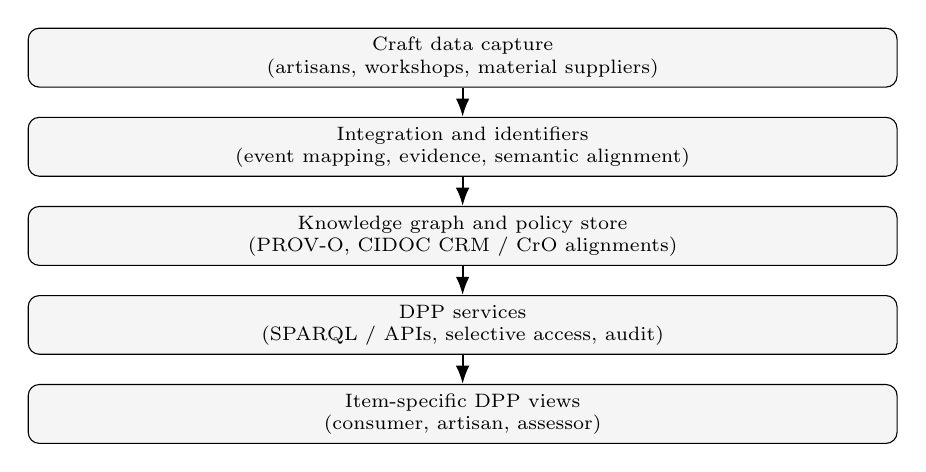
\begin{tikzpicture}[node distance=3.7mm, every node/.style={font=\scriptsize}, box/.style={draw,rounded corners,align=center,minimum width=0.91\columnwidth,minimum height=7mm,fill=gray!8}, arr/.style={-Latex,thick}]
\node[box] (cap) {Craft data capture\\(artisans, workshops, material suppliers)};
\node[box,below=of cap] (integ) {Integration and identifiers\\(event mapping, evidence, semantic alignment)};
\node[box,below=of integ] (kg) {Knowledge graph and policy store\\(PROV-O, CIDOC CRM / CrO alignments)};
\node[box,below=of kg] (api) {DPP services\\(SPARQL / APIs, selective access, audit)};
\node[box,below=of api] (ui) {Item-specific DPP views\\(consumer, artisan, assessor)};
\draw[arr] (cap) -- (integ);
\draw[arr] (integ) -- (kg);
\draw[arr] (kg) -- (api);
\draw[arr] (api) -- (ui);
\end{tikzpicture}
\caption{Proposed AC-DPP architecture (not an implemented system).}
\label{fig:architecture}
\end{figure}

The graph may use SHACL to validate required links, controlled vocabularies, identifiers, and cardinality constraints before exposing a passport \cite{w3c2017shacl}. Verifiable Credentials may optionally convey signed claims from authorized organizations, such as a craft association confirming a particular qualification; however, a valid signature verifies the issuer and integrity of a claim, not the factual truth of the assertion \cite{w3c2025vc}.

\section{Illustrative Scenario and Evaluation Protocol}
\subsection{Worked Scenario}
Consider an illustrative handcrafted ceramic vessel, \texttt{vase-023}, made from locally sourced clay. One artisan prepares and shapes the vessel, another decorates it, and a third carries out firing at a shared kiln. The DPP identifies the item and links it to clay-lot provenance and three sequential activities. Each activity has one or more named or pseudonymous contributors, roles, techniques, and supporting evidence. A consumer can see an authorized product story; a workshop manager can follow lot transformations; an authorized auditor can examine more detailed attestations. This scenario is a design illustration and must not be interpreted as a real case study or measured result.

\subsection{Prospective Evaluation}
A subsequent empirical study should report the following measurable outcomes and compare them with a baseline consisting of workshop/product metadata or a generic unextended provenance model:
\begin{itemize}
\item \textbf{Coverage:} proportion of elicited information requirements represented without ad hoc free-text fields.
\item \textbf{Competency-question completeness:} fraction of benchmark queries with correct answers on a curated gold-standard traceability dataset.
\item \textbf{Trace reconstruction:} precision and recall of material and artisan paths under splits, merges, and multi-artisan activities.
\item \textbf{Interoperability:} successful round-trip mapping to selected PROV-O, CIDOC CRM, and event records, accompanied by an analysis of semantic information lost.
\item \textbf{Data quality and privacy:} SHACL conformance, proportion of restricted facts exposed in public outputs, correction workflows, and consent withdrawal behavior where applicable.
\item \textbf{Usability:} task completion time, error rate, and perceived effort for artisans with different levels of digital literacy.
\end{itemize}

The evaluation should include multiple production patterns: one maker performing all tasks, multiple makers performing sequential tasks, shared activities, changing material lots, and contested attributions. It should also document the size and provenance of its dataset, expert annotation protocol, recruitment procedure, query set, and threats to validity. No quantitative results are yet available for these metrics.

\section{Discussion}
The proposed contribution is principally the integration of mature semantic resources into an item-centred, contribution-aware DPP pattern. Provenance is multidimensional: an item can have a reliable material trail yet incomplete attribution of its makers; conversely, a well-documented artisan history does not establish a material's origin. Keeping these dimensions separate but linked supports more precise queries and disclosure policies.

Semantic standard reuse limits unnecessary reinvention, but does not eliminate conceptual differences. For example, PROV-O speaks generically of agents and activity associations; CIDOC CRM places the creation and modification of cultural objects in an event-oriented historical account; CrO captures the specifics of craft practice. Mappings should therefore distinguish strict equivalence, specialization, and application-level bridging relations.

An equally important limitation is the distinction between \emph{asserted}, \emph{attested}, and \emph{independently verified} provenance. Self-reported contributions can still be valuable, but should not be advertised as independently authenticated. A transparent data model should indicate who entered or certified each claim and how corrections are managed. Attribution may also be contested among contributors; the system should permit competing claims rather than silently overwriting prior statements.

Finally, recognition of artisans must not translate into obligatory publication of personal histories. Privacy, consent where appropriate, legitimate purposes, minimal disclosure, and the intellectual-property interests of artisans should be incorporated during design. Not every workshop will be able to afford detailed capture and curation; adoption requires lightweight workflows and evidence models appropriate for micro-enterprises.

\section{Conclusion and Future Work}
This paper has outlined an Artisan-Centred Digital Product Passport connecting material provenance, product transformations, and the contributions of individual artisans. Its proposed contribution is to reuse PROV-O, CIDOC CRM, and craft-domain semantics through a contribution-centred information pattern, and to connect this pattern to DPP identification, presentation, and governance services. A structured set of requirements and competency questions, architecture, and prospective evaluation protocol are provided without claiming an implemented system or completed experimental validation.

Future work includes validating the requirements with artisans, publishing a documented ontology profile and crosswalk, implementing a demonstrator for at least two craft domains, and conducting comparative evaluation of traceability, semantic interoperability, privacy, and usability. Such a programme could determine whether artisan-centred provenance becomes a useful, interoperable extension of emerging DPP ecosystems.

\bibliographystyle{IEEEtran}
\bibliography{refs}
\end{document}
